\hthree{Beispiele}
\hfour{Vergleich: Light- und Dark-Theme}

Die Zelia App lässt sich sowohl im Light- als auch im Dark-Theme anzeigen (Siehe Abbildung \ref{fig:theme}). Dafür werden Media-Queries (Siehe Kapitel \ref{sec:mediaQueries}) verwendet, welche das Theme des Browsers abfragen (Siehe Code \ref{code:theme}). 
Die jeweiligen Farben werden in CSS-Variablen gespeichert. Dadurch müssen die Farben nur einmal in einer Media-Query angepasst werden und können nun für jedes Element verwendet werden. 

\begin{figure}[H]
    \begin{subfigure}[c]{0.5\textwidth}
        \centering
        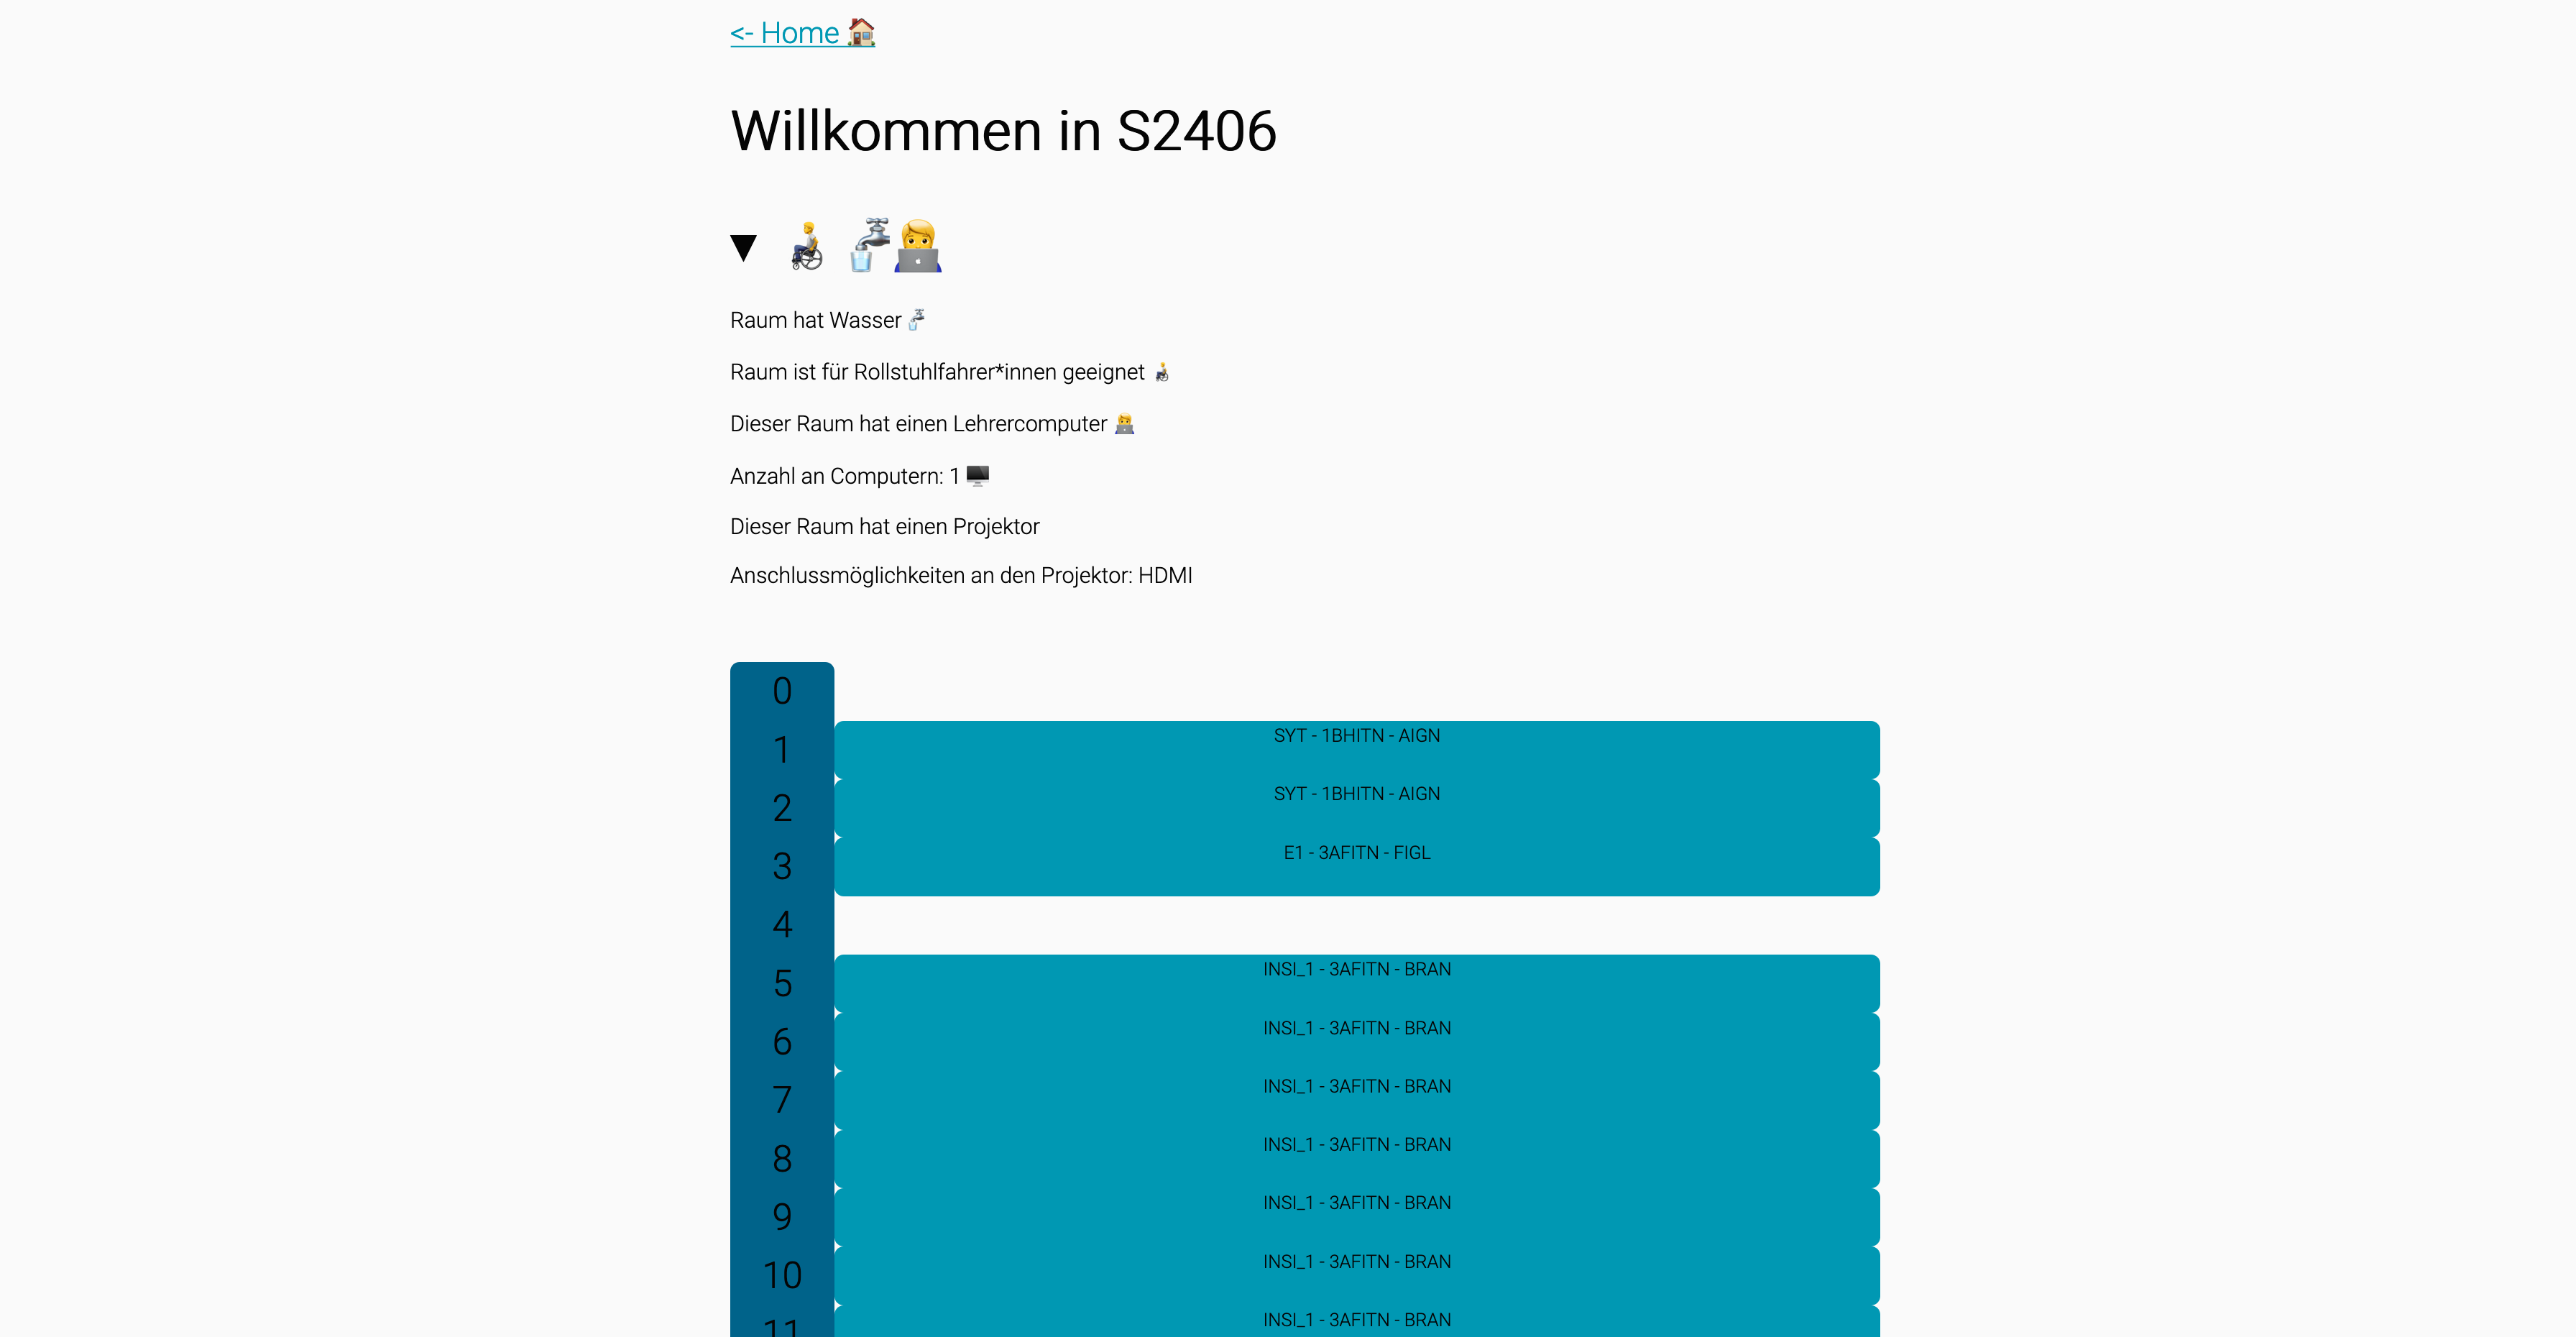
\includegraphics[width=\textwidth]{media/ResponsiveDesign/ZeliaDesktop.png}
        \caption{Helles Theme}
    \end{subfigure} \hfill
    \begin{subfigure}[c]{0.5\textwidth}
        \centering
        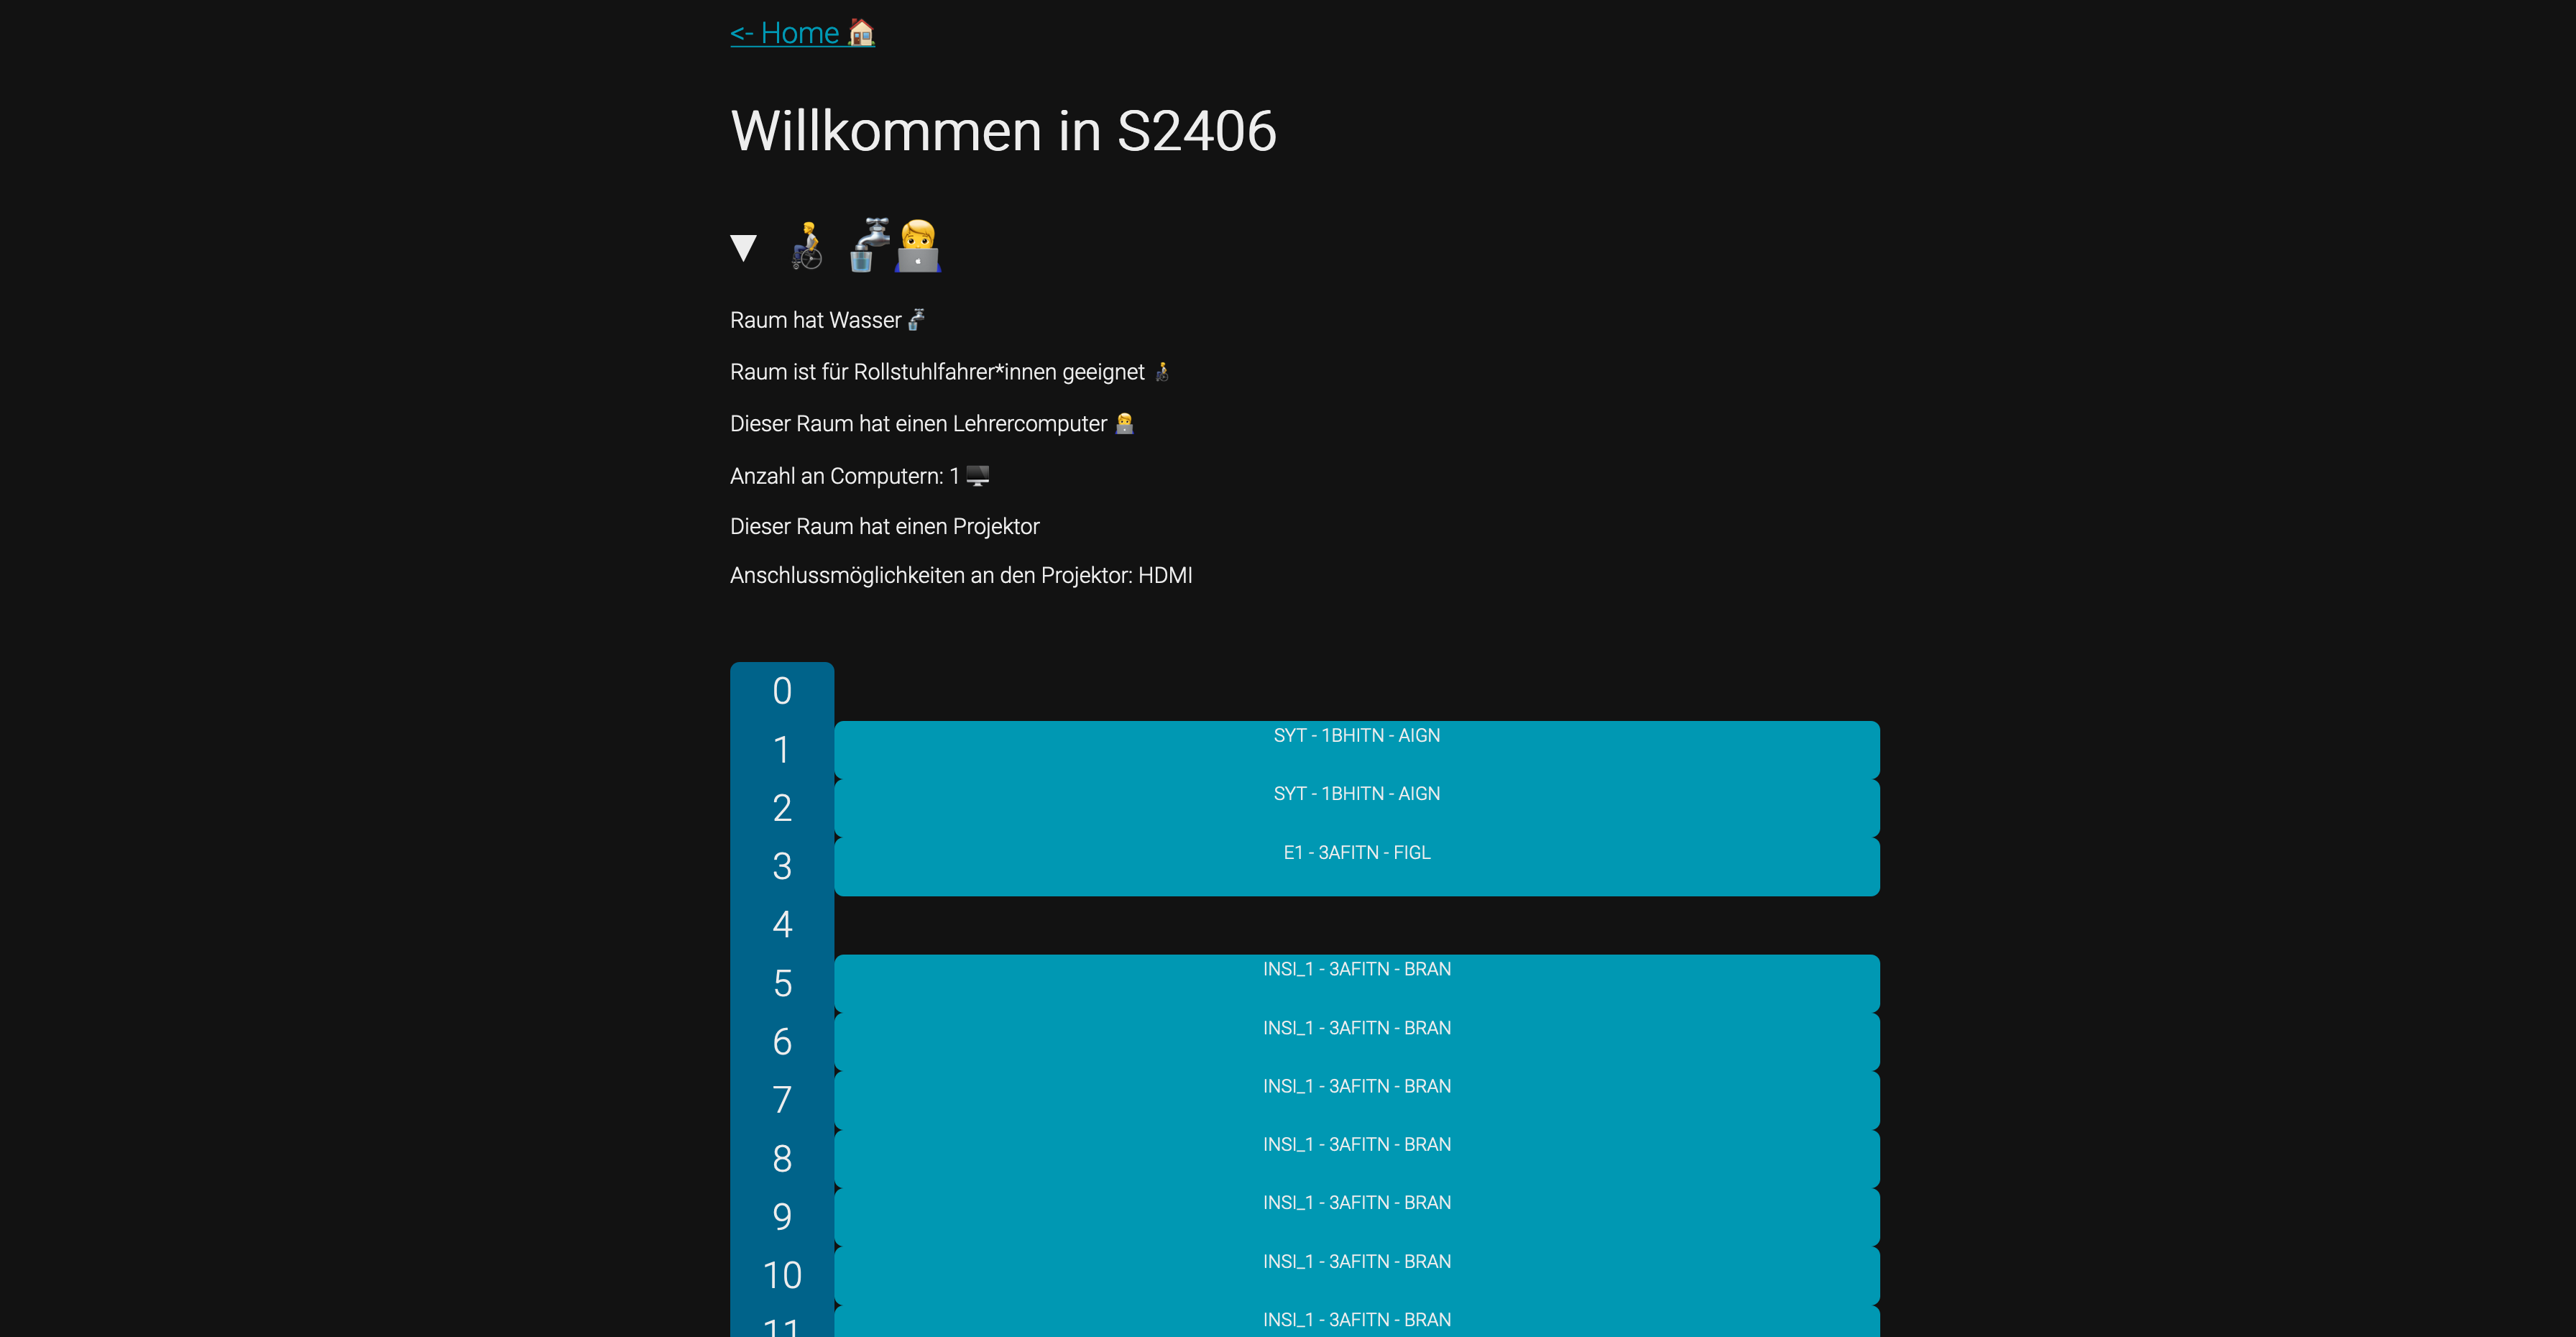
\includegraphics[width=\textwidth]{media/ResponsiveDesign/ZeliaDesktopDark.png}
        \caption{Dunkles Theme}
    \end{subfigure}
    \caption{Gegenüberstellung vom hellen und dunklen Theme}
    \label{fig:theme}
\end{figure}

\css[code:theme]{code/ResponsiveDesign/theme.css}{Anpassung der Farben anhand des Themes}

\clearpage
\hfour{Vergleich: Mobil und Desktop}

Da Zelia sowohl am Desktop als auch am Mobil genutzt verwendbar sein soll, wird mithilfe der Clamp-Funktion (Siehe Kapitel \ref{sec:clamp}) das Design für die verschiedenen Bildschirmgrößen angepasst (Siehe Abbildung \ref{fig:info}).


\begin{figure}[H]
    \begin{subfigure}[c]{0.65\textwidth}
        \centering
        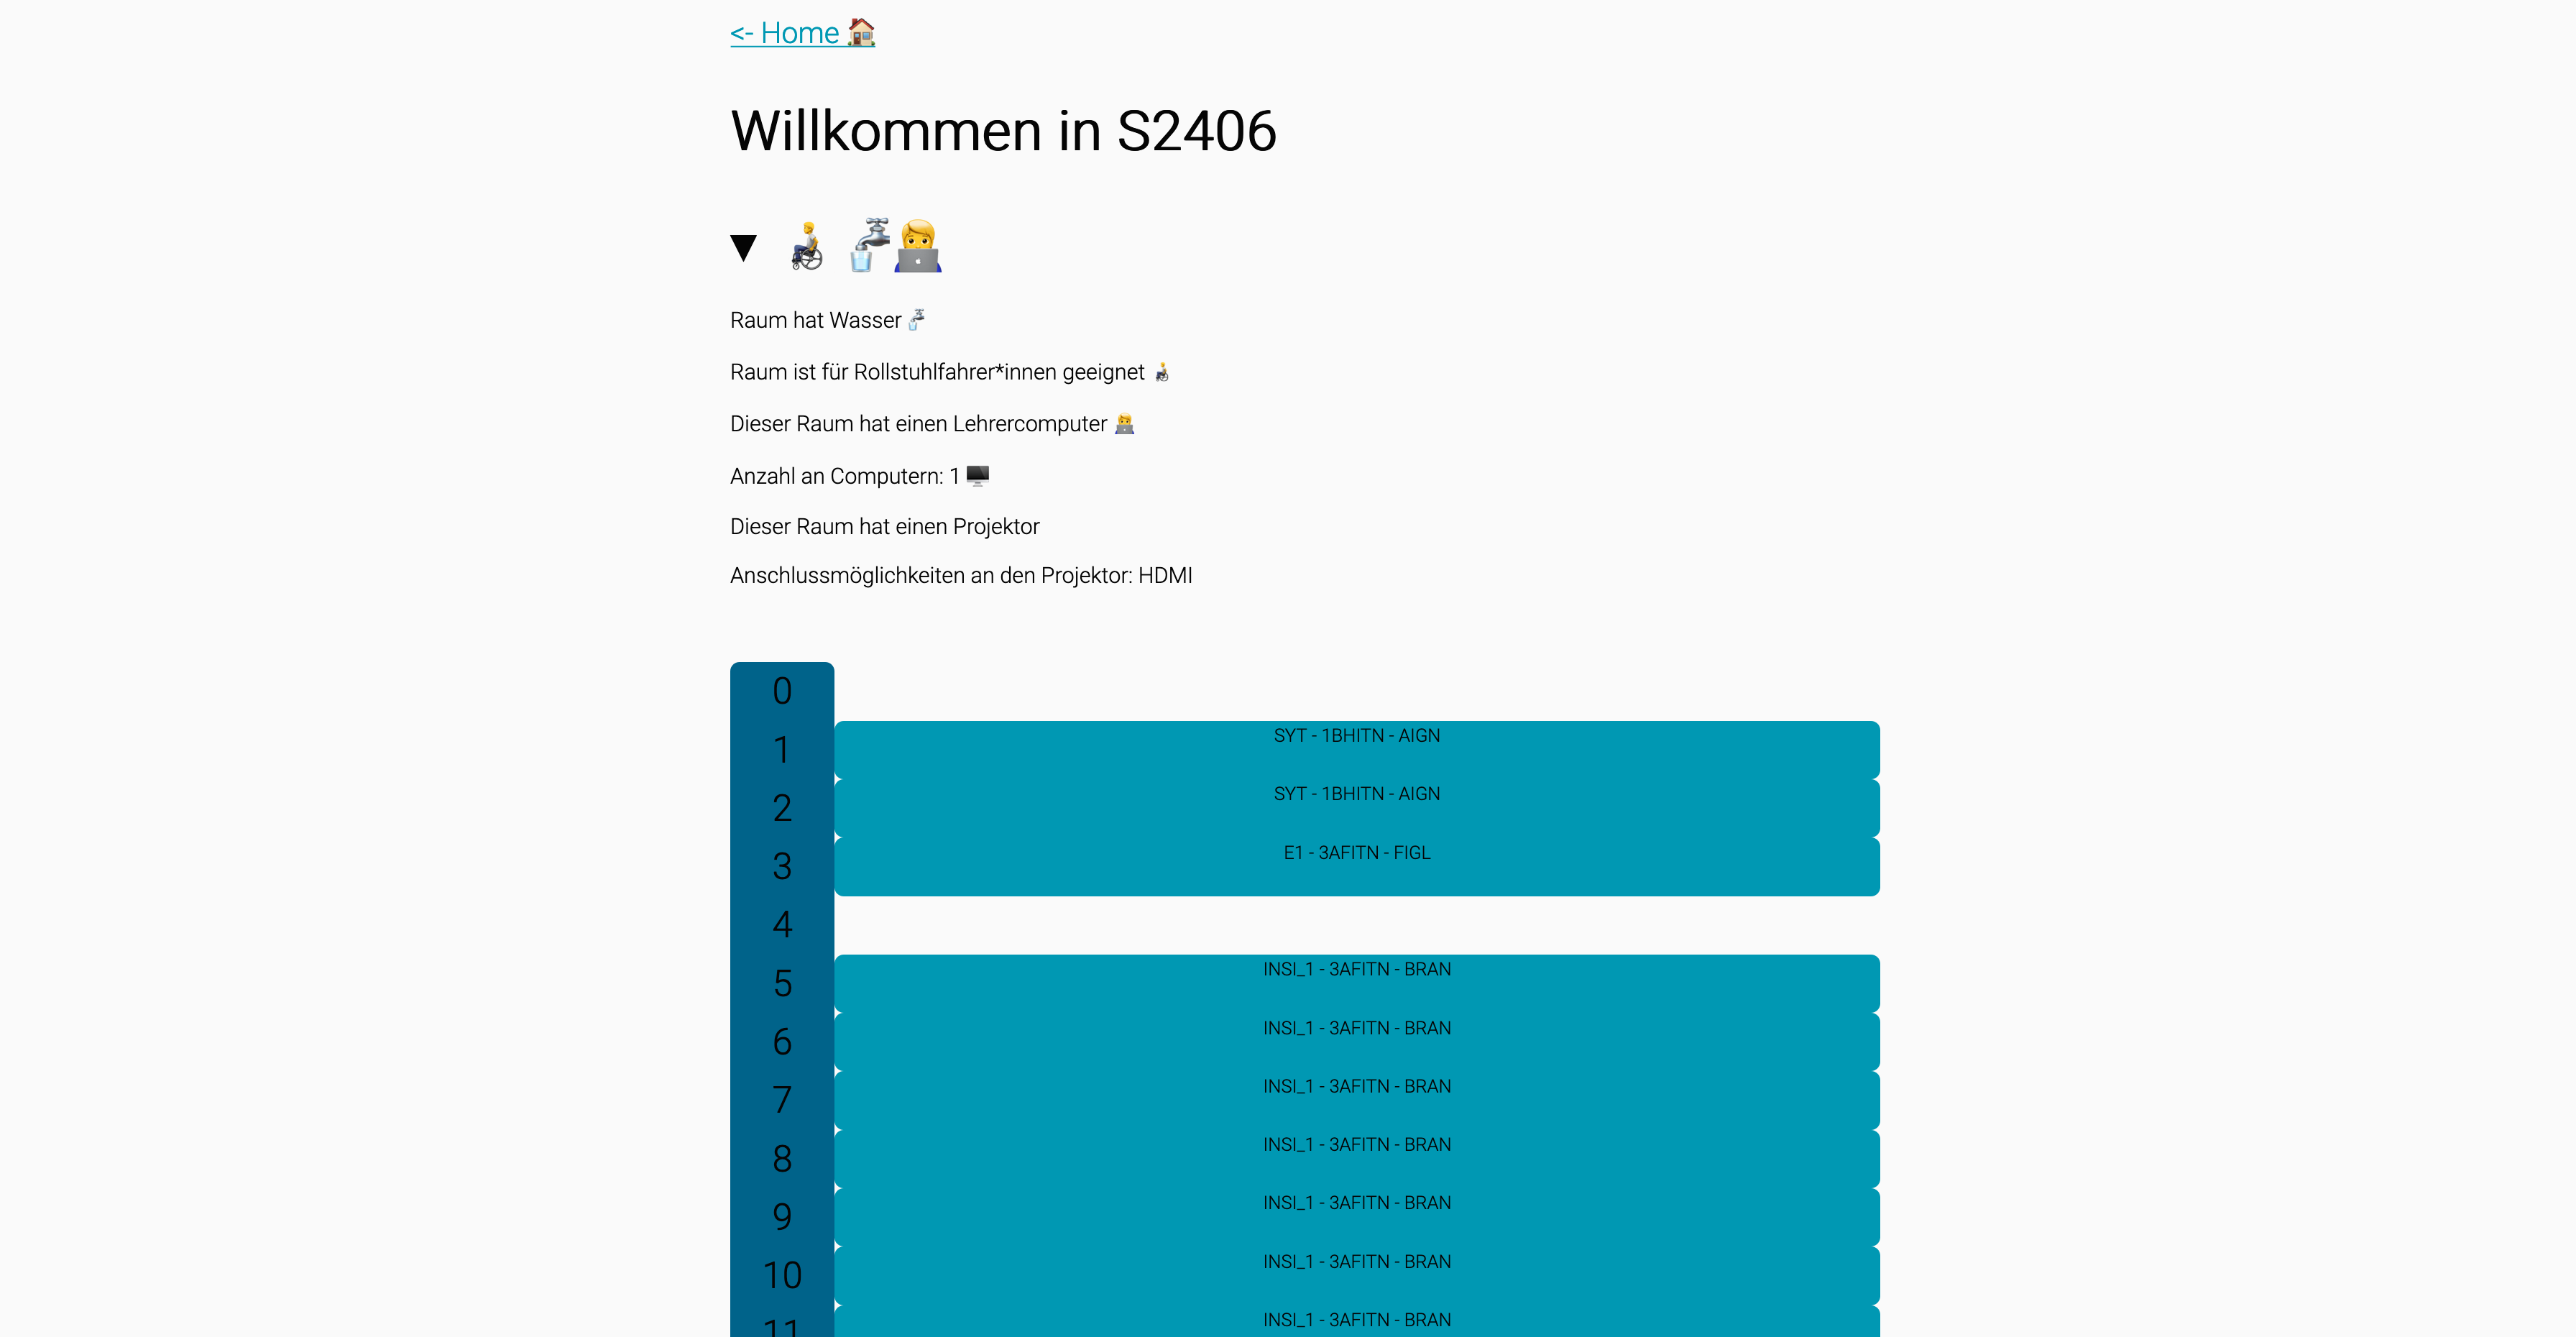
\includegraphics[width=\textwidth]{media/ResponsiveDesign/ZeliaDesktop.png}
        \caption{Rauminfo (Desktop)}
    \end{subfigure} \hfill
    \begin{subfigure}[c]{0.35\textwidth}
        \centering
        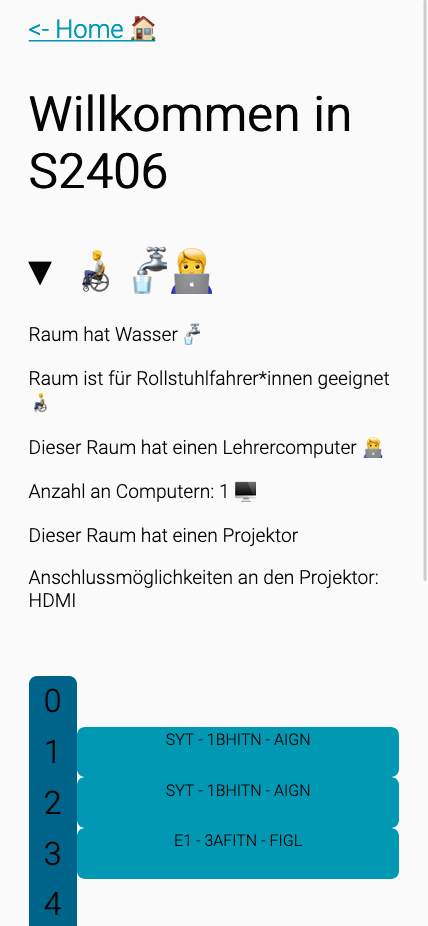
\includegraphics[width=\textwidth]{media/ResponsiveDesign/ZeliaMobile.png}
        \caption{Rauminfo (Mobil)}
    \end{subfigure}
    \caption{Vergleich von Desktop- und Mobile-Versionen der Rauminformation}
    \label{fig:info}
\end{figure}

Damit die Raumnummer auf den Mobilgeräten mittels OCR (Siehe Kapitel \ref{sec:ocr}) eingelesen werden kann, wird der "Kamera öffnen"-Button (Siehe Abbildung \ref{fig:homeMobile}) dafür angezeigt oder ausgeblendet, je nach dem, ob das Gerät ein Mobilgerät ist (Siehe Abbildung \ref{fig:home}).

\begin{figure}[H]
    \begin{subfigure}[c]{0.65\textwidth}
        \centering
        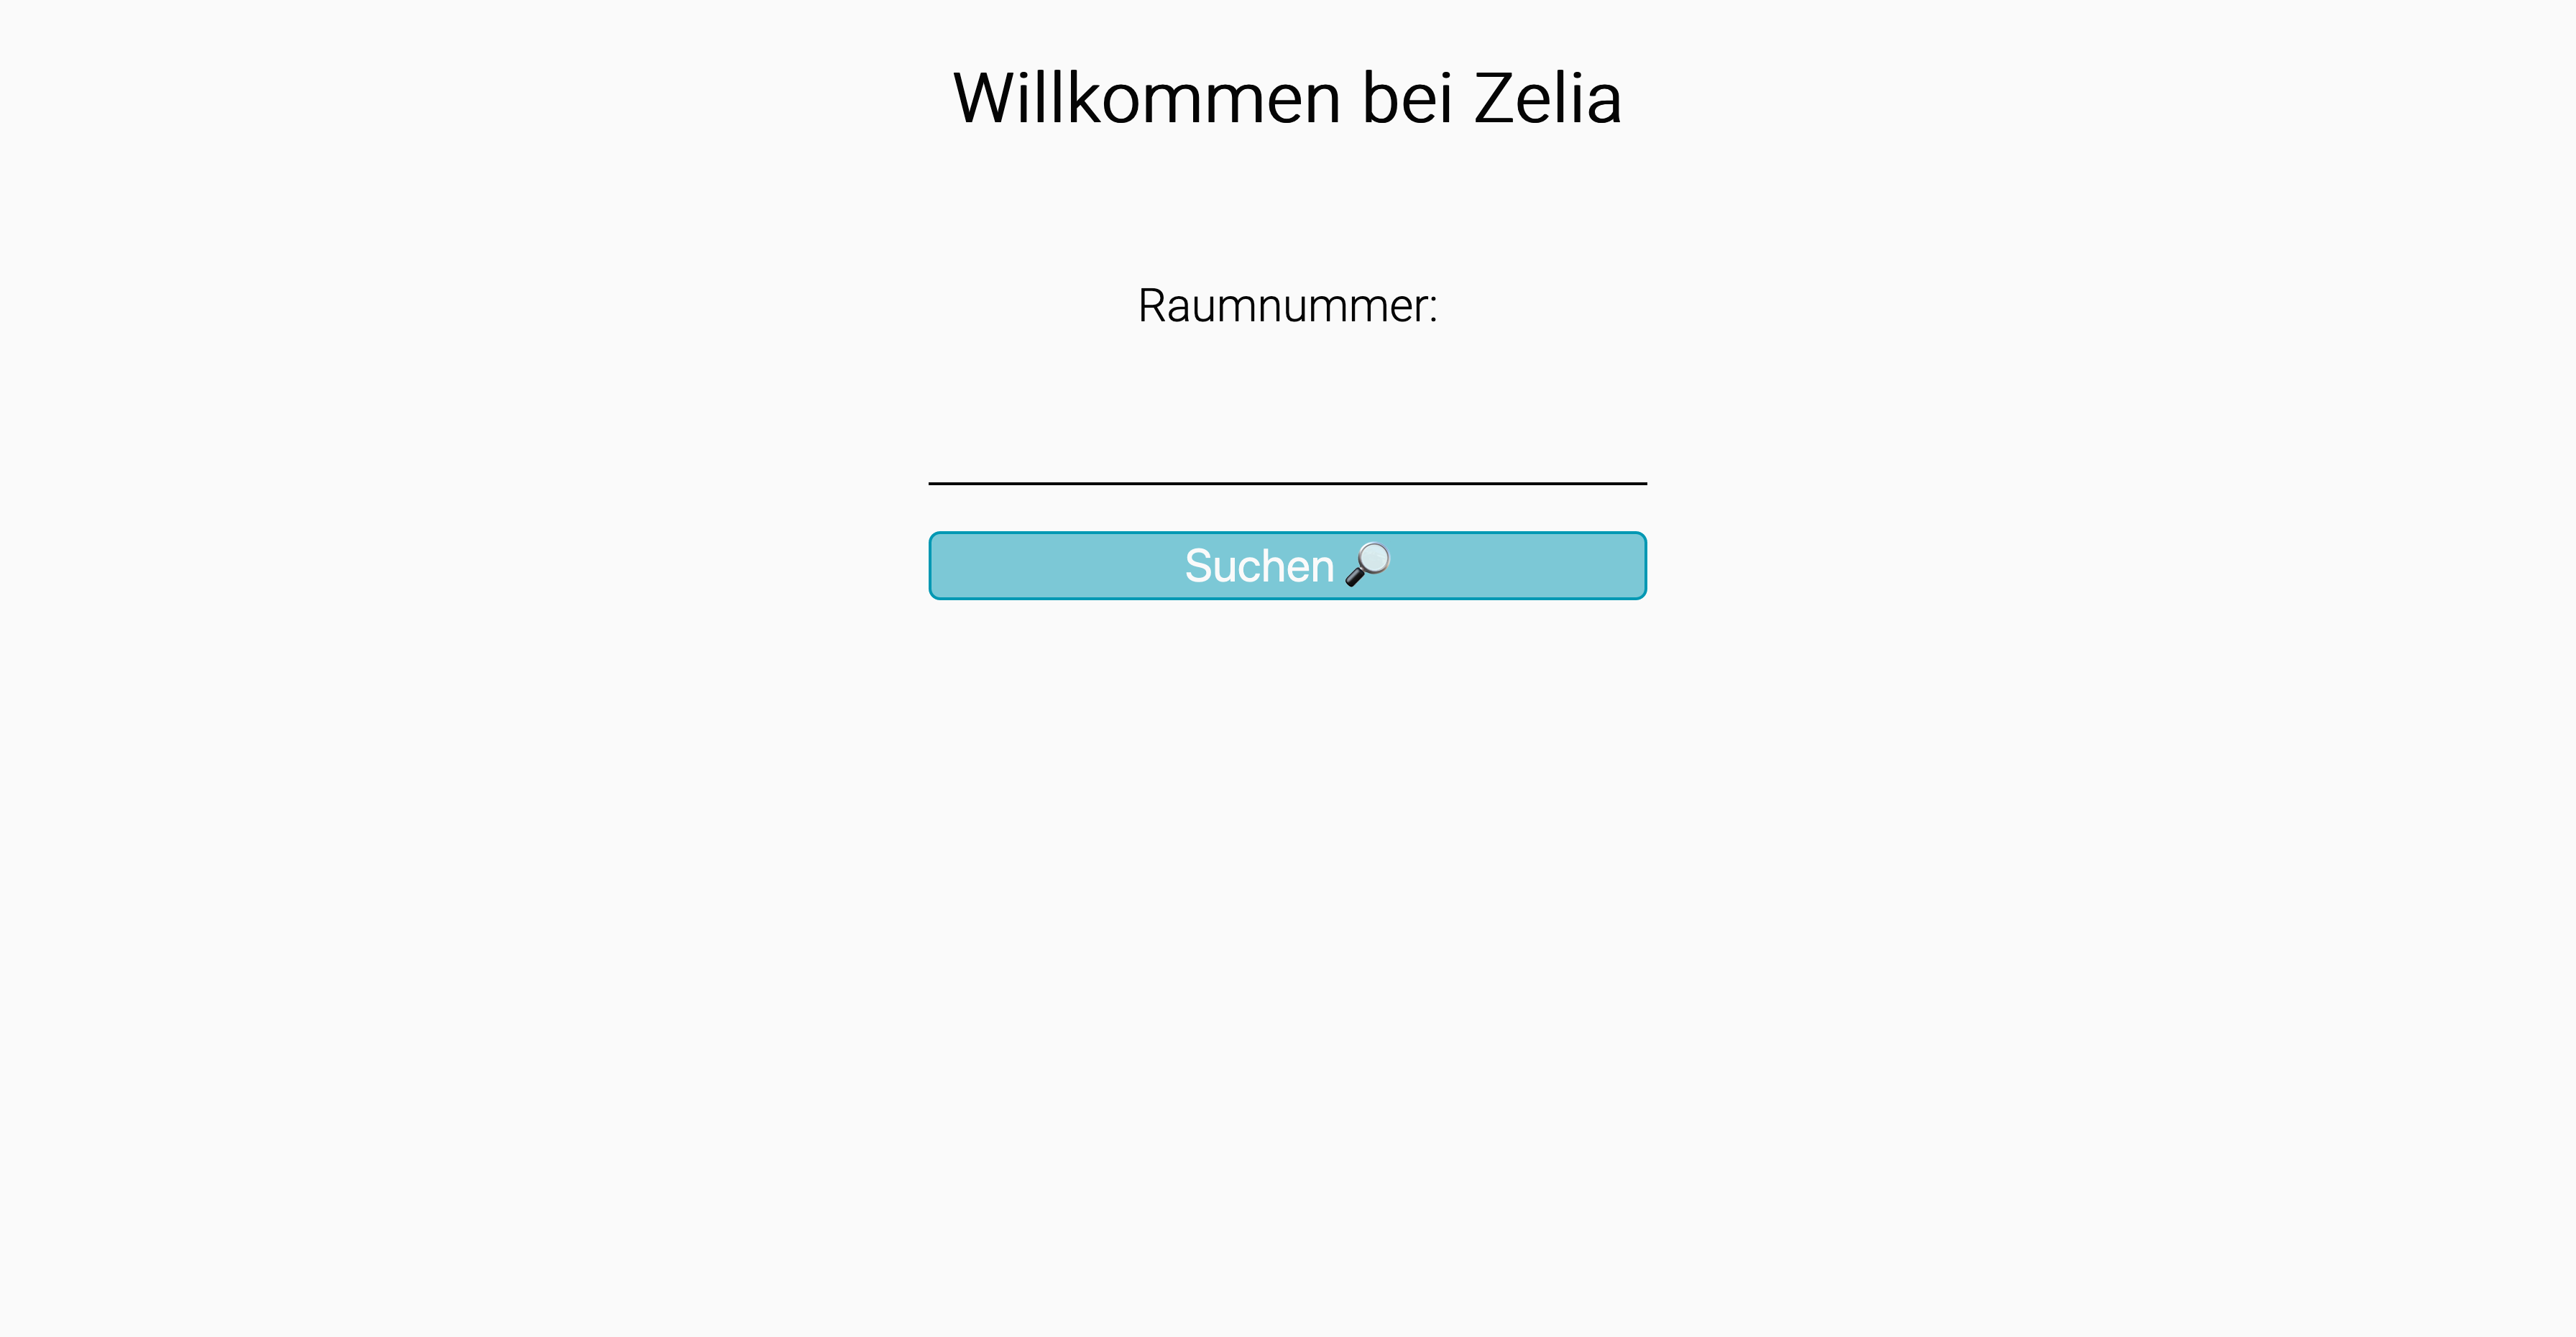
\includegraphics[width=\textwidth]{media/ResponsiveDesign/ZeliaHome.png}
        \caption{Startseite (Desktop)}
    \end{subfigure} \hfill
    \begin{subfigure}[c]{0.35\textwidth}
        \centering
        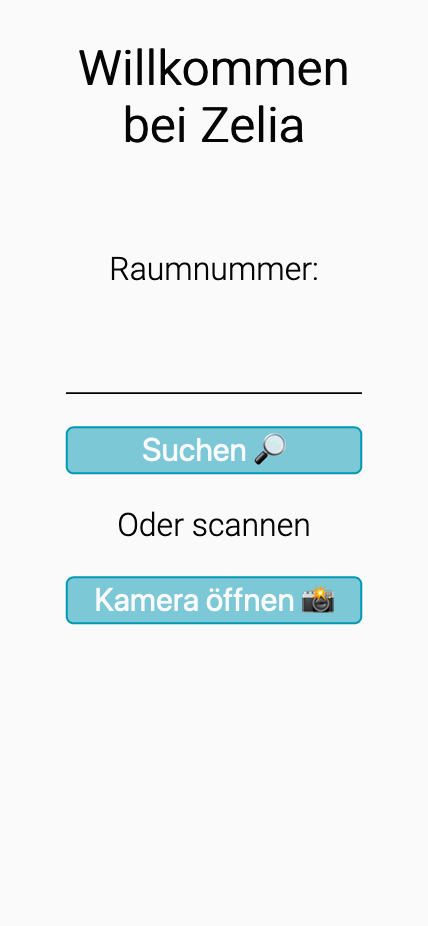
\includegraphics[width=\textwidth]{media/ResponsiveDesign/ZeliaHomeMobile.png}
        \caption{Startseite (Mobil)}
        \label{fig:homeMobile}
    \end{subfigure}
    \caption{Vergleich von Desktop- und Mobile-Versionen der Startseite}
    \label{fig:home}
\end{figure}